\documentclass[10pt,twocolumn,letterpaper]{article}
\usepackage[pagenumbers]{cvpr}

\usepackage{graphicx}
\usepackage{amsmath}
\usepackage{amssymb}
\usepackage{booktabs}
\definecolor{cvprblue}{rgb}{0.21,0.49,0.74}
\usepackage[breaklinks,colorlinks,allcolors=cvprblue]{hyperref}
\graphicspath{{../figures/}}

\title{Project 4 - Object detection}

\author{Oliver Colmer\\
{\tt\small s245647@dtu.dk}
\and
Philippa Bagger\\
{\tt\small s246103@dtu.dk}
\and
Gustav Bellaiche\\
{\tt\small s245243@dtu.dk}
\and
Eren Chaglar\\
{\tt\small s245735@dtu.dk}
}

\begin{document}
\maketitle

%--------------------------------------------------------------------
\section{Introduction}
Potholes have a large impact on road safety, and a system that detects them automatically could be mounted on cars or robots that scan the roads. This project builds such a detector from scratch following R-CNN, in three steps: object proposals are extracted, evaluated and labelled (4.1), a CNN is fine-tuned to classify the proposals (4.2), and the network is applied to the test images followed by non-maximum suppression (NMS) and evaluation with Average Precision (AP) (4.3).

%--------------------------------------------------------------------
\section{Background}
\subsection{R-CNN style detection}
R-CNN splits detection into \emph{where} and \emph{what}. A class-agnostic method proposes a few thousand boxes per image. Each box is cropped, warped to a fixed size and classified by a CNN into $N$ object classes or background ($N{+}1$ classes, here $N=1$). Two boxes are compared by their Intersection over Union, $\text{IoU}=\frac{\text{area of intersection}}{\text{area of union}}$, and a prediction counts as correct if IoU $\ge 0.5$ with a GT box. Since many proposals cover the same object, the raw detections are post-processed with non-maximum suppression (NMS): (1) select the highest-scoring remaining box, (2) eliminate lower-scoring boxes with IoU $>$ threshold to it, (3) repeat while boxes remain. NMS is class-specific, which is trivial here with one class. It can fail in cluttered images with highly overlapping objects.

\begin{figure*}[t]
\centering
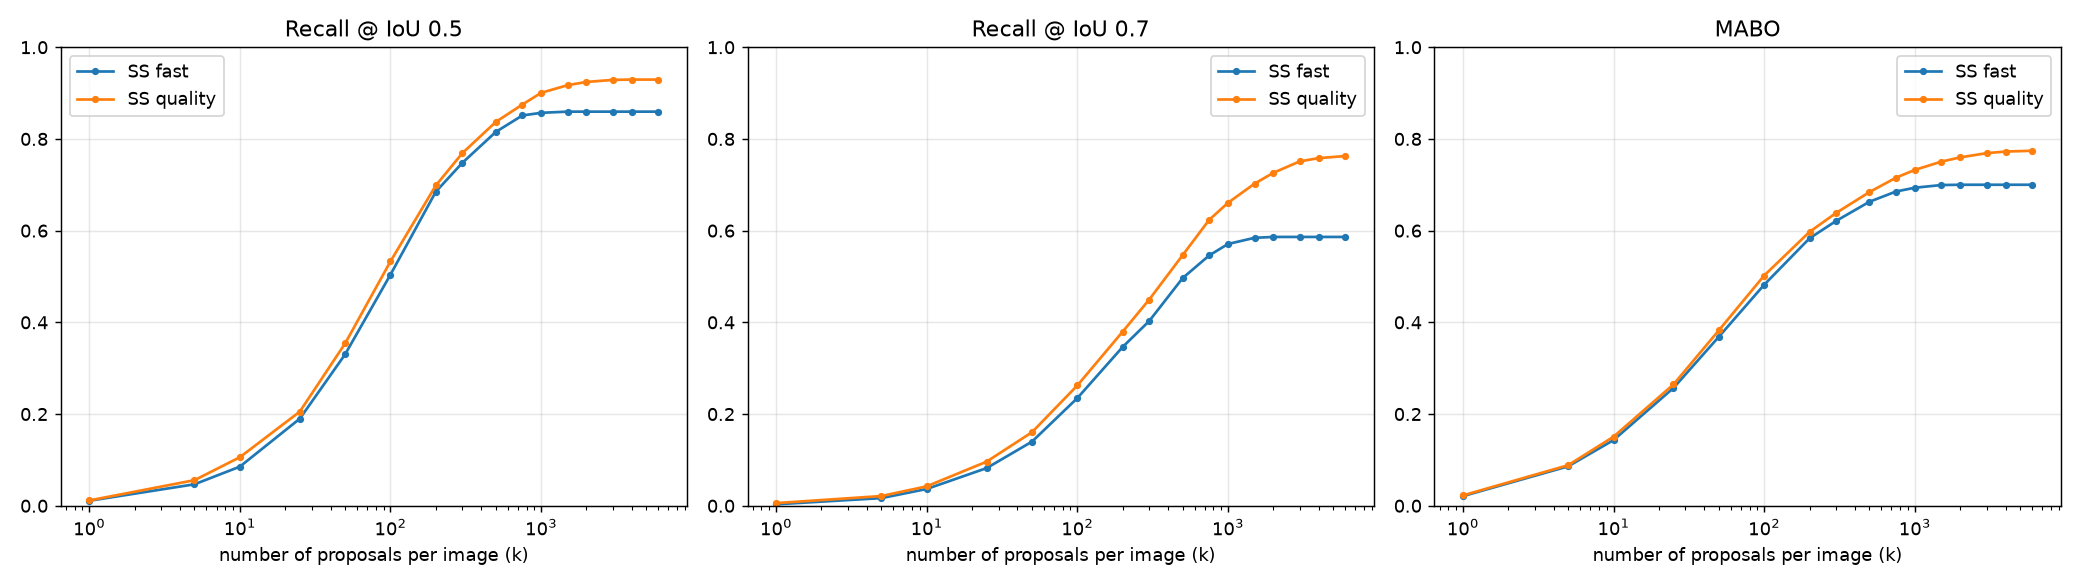
\includegraphics[width=0.72\linewidth]{proposal_recall.png}
\caption{Proposal recall at IoU 0.5 and 0.7 and MABO on the training images \vs the number of proposals per image.}
\label{fig:recall}
\end{figure*}

\subsection{Selective Search}
Selective Search is a bottom-up segmentation that merges regions at multiple scales; every region is converted to a box, giving a class-agnostic set of proposals with high recall. The \emph{fast} mode uses fewer colour spaces and similarity measures than the \emph{quality} mode and gives fewer proposals.

\subsection{Data}
The Potholes dataset has 665 images, mostly $400\times400$ or ${\sim}450\times300$\,px, with 1740 potholes annotated as boxes in PascalVOC XML. An image contains 2.6 potholes on average and up to 19, and the boxes are small (median $80\times40$\,px).

%--------------------------------------------------------------------
\section{Method}
\noindent\textbf{Data and preprocessing.}
Since \texttt{splits.json} is missing, the images are sorted by file name and split with \texttt{train\_test\_split(test\_size=0.1, random\_state=42)} (598 train / 67 test), as agreed across groups. 10\% of the training images are split off as validation set with the same seed. Two boxes with a side of $\le 2$\,px were removed and one box extending past the image border was clipped.

\noindent\textbf{Proposals.}
We use Selective Search from OpenCV in both modes; as recommended in the lecture, images are resized so that the largest side is at most 500\,px (102 of 665 images), and the boxes are scaled back. The fast mode takes 1.2\,s and gives 764 boxes per image on average, the quality mode 4.0\,s and 2502 boxes. Proposals are evaluated by the recall, \ie the fraction of ground-truth (GT) boxes covered by one of the top-$k$ proposals with IoU $\ge 0.5$ or $0.7$, and by the mean average best overlap (MABO).

\noindent\textbf{Labelling.}
Each proposal $A$ (after removing duplicates and boxes with a side $<4$\,px) is labelled from $\max_i \text{IoU}(A,\text{GT}_i)$: \emph{background} if it is $<k_1$ and \emph{pothole} if it is $\ge k_2$. We use $k_1=0.3$, $k_2=0.5$; proposals in between are discarded, so the classifier is not trained on borderline crops. The GT boxes are added as extra positives.

\noindent\textbf{Architecture.}
We fine-tune an ImageNet-pretrained ResNet-50. Every proposal is enlarged by 10\% on each side for context, cropped and warped to $224\times224$. The final layer is replaced by two heads: a classifier with $N{+}1=2$ outputs and a box regressor predicting a transform $(t_x,t_y,t_w,t_h)$ from a proposal with centre $(p_x,p_y)$, width $p_w$ and height $p_h$ to the target box $b$ (its matched GT box),
\begin{equation*}
t_x=\tfrac{b_x-p_x}{p_w},\; t_y=\tfrac{b_y-p_y}{p_h},\; t_w=\log\tfrac{b_w}{p_w},\; t_h=\log\tfrac{b_h}{p_h}.
\end{equation*}
The transform is relative to the proposal size, since the CNN does not see absolute size or position after cropping. The loss is cross-entropy plus a smooth-$L_1$ box loss on the positives only.

\noindent\textbf{Dataloader and class imbalance.}
The labelling gives 25 background crops per pothole crop, so always predicting background would already give 96\% accuracy. Following the lecture, we sample proposals so that each batch has 75\% background and 25\% potholes (32 of 128), drawn with replacement. Every positive is thus seen many times, while the large and redundant background pool is subsampled differently in every batch. Crops are cut on the fly, with horizontal flips as augmentation.

\noindent\textbf{Training.}
AdamW with a one-cycle schedule is used (\cref{tab:setup}). After each epoch, the model is evaluated on the validation positives and 15k random background crops, and the checkpoint with the highest proposal-level AP is kept.

\noindent\textbf{Inference and NMS.}
For a test image, the top-2000 proposals are scored by the softmax probability of \emph{pothole} and refined with the predicted offsets. We implemented greedy NMS ourselves (it returns exactly the same boxes as \texttt{torchvision.ops.nms}), with the IoU threshold chosen on the validation images and at most 100 detections per image.

\noindent\textbf{Metrics.}
We use $\text{Precision}=\frac{TP}{TP+FP}$ and $\text{Recall}=\frac{TP}{TP+FN}$, plus accuracy and balanced accuracy (mean of the per-class recalls) for the classifier. For detection we implemented Average Precision: all test detections after NMS are sorted by decreasing score; a detection that matches a GT box with IoU $\ge 0.5$ is marked positive and the GT box is removed, otherwise it is negative, so duplicates count as false positives. AP is the area under the resulting precision-recall curve, \ie the sum of the precisions at the true positives divided by the number of GT boxes. With one class, mAP equals AP. We also report AP with the stricter IoU 0.75.

\begin{table}[t]
\centering
\footnotesize
\setlength{\tabcolsep}{4pt}
\begin{tabular}{@{}ll@{}}
\toprule
Train/val/test images & 538 / 60 / 67 \\
Proposals & SS quality, top $k=2000$ \\
Train crops (pothole / bg.) & 31\,723 / 801\,480 \\
Val crops (pothole / bg.) & 3\,794 / 82\,080 \\
\midrule
Backbone, input & ResNet-50, $224\times224$ \\
Batch & 128 (25\% positives) \\
Optimiser & AdamW, lr $10^{-4}$ (heads $10^{-3}$) \\
Schedule & one-cycle, 10 epochs $\times$ 300 it. \\
Training time & 9 min on a V100 \\
Seed & split 42, training 0 \\
\bottomrule
\end{tabular}
\caption{Experimental setup.}
\label{tab:setup}
\end{table}

%--------------------------------------------------------------------
\section{Experiments}
\noindent\textbf{Object proposals.}
\cref{fig:recall} shows the proposal quality on the training images. The fast mode saturates at 86\% recall@0.5 after about 1000 proposals, because it produces no more boxes. The quality mode improves up to about 2000 proposals (92.4\%) and gains little afterwards (92.9\% at 6000). The difference is larger at IoU 0.7 (59\% \vs 73\% at $k=2000$), so the quality mode also gives better-localised boxes. We therefore use the quality mode with $k=2000$. About 7\% of the potholes are never covered by a proposal, which is an upper bound on the recall of the detector. The labelled training split has 883\,560 background and 35\,517 pothole samples (\cref{fig:labels}).


\begin{figure}[t]
\centering
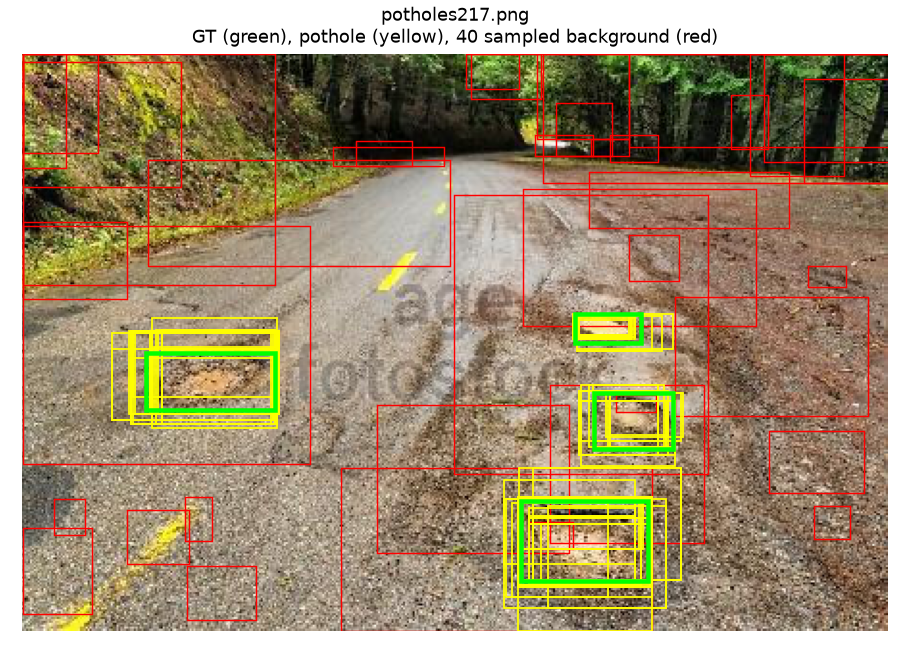
\includegraphics[width=0.6\linewidth]{labeled_proposals_example.png}
\caption{A training image with GT (green), pothole proposals (yellow) and 40 of the 1400 background proposals (red).}
\label{fig:labels}
\end{figure}

\begin{figure}[t]
\centering
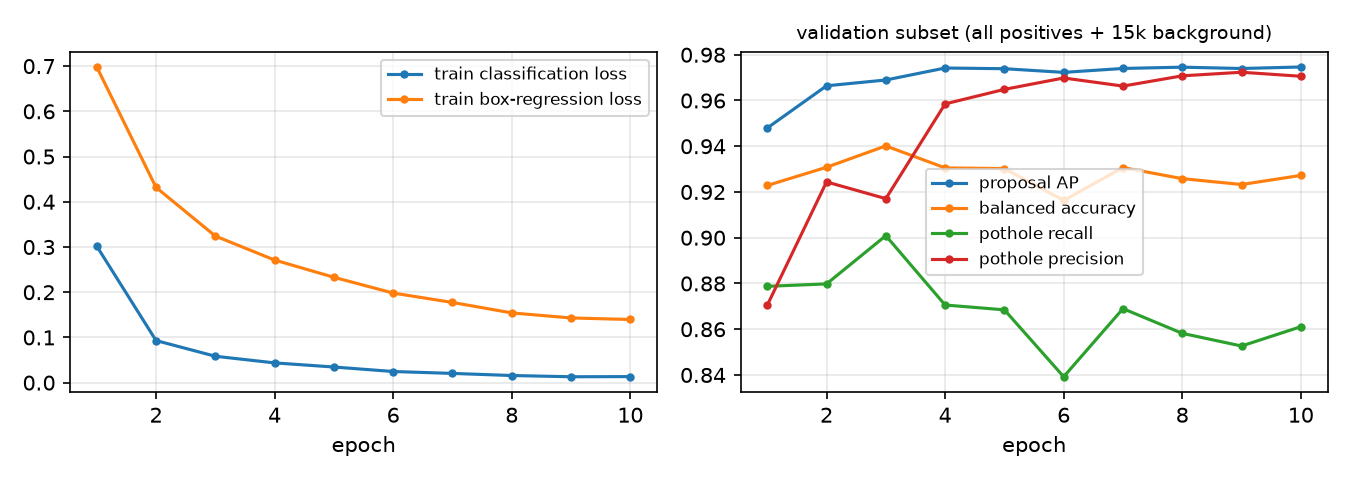
\includegraphics[width=\linewidth]{training_curves.png}
\caption{Training losses (left) and validation metrics on the validation subset (right) per epoch.}
\label{fig:train}
\end{figure}

\noindent\textbf{Proposal classification.}
\cref{fig:train} shows that the training loss keeps decreasing, while the validation metrics plateau after 4--5 epochs, so longer training would mainly overfit. \cref{tab:cls} reports the final model on the \emph{full} validation set (4.4\% potholes). The accuracy of 98.7\% is misleading, since always predicting background gives 95.6\%. At threshold 0.5 the classifier finds 86\% of the pothole crops with 84\% precision, and misclassifies only 0.7\% of the background crops. With 1400 background crops per image this is still about 10 false positives per image, which NMS and the score ranking have to handle.

\begin{table}[t]
\centering
\footnotesize
\setlength{\tabcolsep}{3.5pt}
\begin{tabular}{@{}cccccc@{}}
\toprule
Thr. & Acc & Bal.\ acc & Pothole rec. & Pothole prec. & Bg.\ rec. \\
\midrule
0.5 & .987 & \textbf{.927} & \textbf{.861} & .844 & .993 \\
0.9 & .988 & .891 & .784 & \textbf{.928} & \textbf{.997} \\
\bottomrule
\end{tabular}
\caption{Proposal classification on the full validation set (3\,794 pothole, 82\,080 background crops) for two thresholds.}
\label{tab:cls}
\end{table}

\begin{table}[t]
\centering
\footnotesize
\setlength{\tabcolsep}{3.2pt}
\begin{tabular}{@{}lccccccc@{}}
\toprule
NMS IoU threshold & 0.1 & 0.2 & 0.3 & 0.4 & 0.5 & 0.6 & 0.7 \\
\midrule
w/o box reg. & .587 & \textbf{.604} & .597 & .571 & .491 & .383 & .270 \\
with box reg. & .680 & .679 & .685 & \textbf{.690} & .679 & .656 & .592 \\
\bottomrule
\end{tabular}
\caption{Validation AP@0.5 for different NMS IoU thresholds, used to choose the threshold for the test set.}
\label{tab:nms}
\end{table}

\noindent\textbf{Object detection.}
\cref{tab:ap} and \cref{fig:pr} show the test results. Without NMS, AP@0.5 is only 0.067, because every pothole is covered by many overlapping high-scoring proposals, and all but one count as false positives. NMS raises AP@0.5 to 0.585. The best NMS threshold on the validation set is 0.2 without box regression and 0.4 with it (\cref{tab:nms}), since without regression many loose boxes around the same pothole survive a higher threshold. Box regression adds 7 points AP@0.5 and triples AP@0.75 (0.103 $\to$ 0.303), because the boxes are better localised. It also allows the higher NMS threshold, which lifts the maximum recall from 0.75 to 0.89, close to the proposal upper bound of 0.92. The final detector reaches AP@0.5 $=$ 0.660.

\begin{table}[t]
\centering
\footnotesize
\setlength{\tabcolsep}{3pt}
\begin{tabular}{@{}lcccc@{}}
\toprule
Method & AP$_{50}$ & AP$_{75}$ & Max rec. & Det./img \\
\midrule
No NMS & .067 & .033 & .922 & 1568 \\
NMS 0.2 & .585 & .103 & .749 & 99 \\
NMS 0.4 + box reg. & \textbf{.660} & \textbf{.303} & .888 & 100 \\
\bottomrule
\end{tabular}
\caption{Detection results on the test set (67 images, 179 potholes).}
\label{tab:ap}
\end{table}

\begin{figure}[t]
\centering
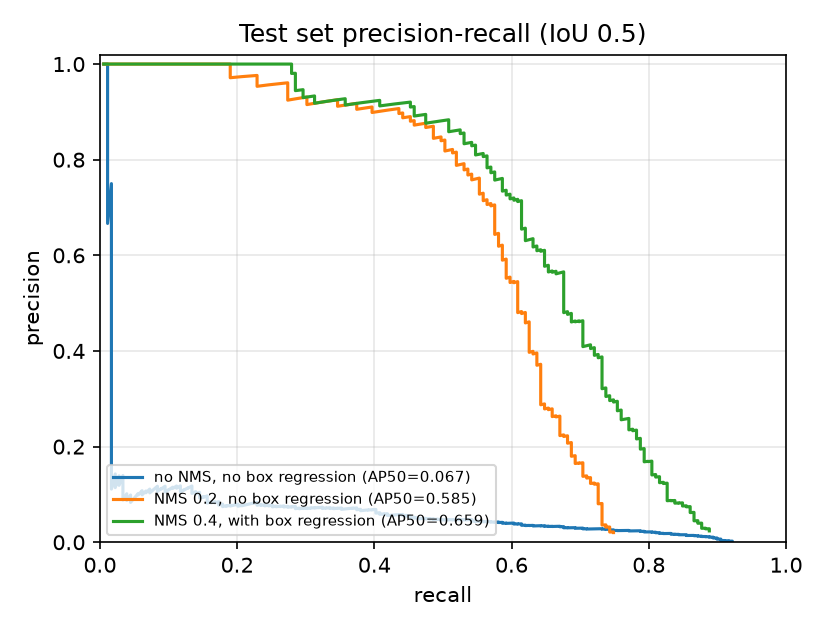
\includegraphics[width=0.7\linewidth]{test_pr_curve.png}
\caption{Precision-recall curves on the test set at IoU 0.5.}
\label{fig:pr}
\end{figure}

\begin{figure}[t]
\centering
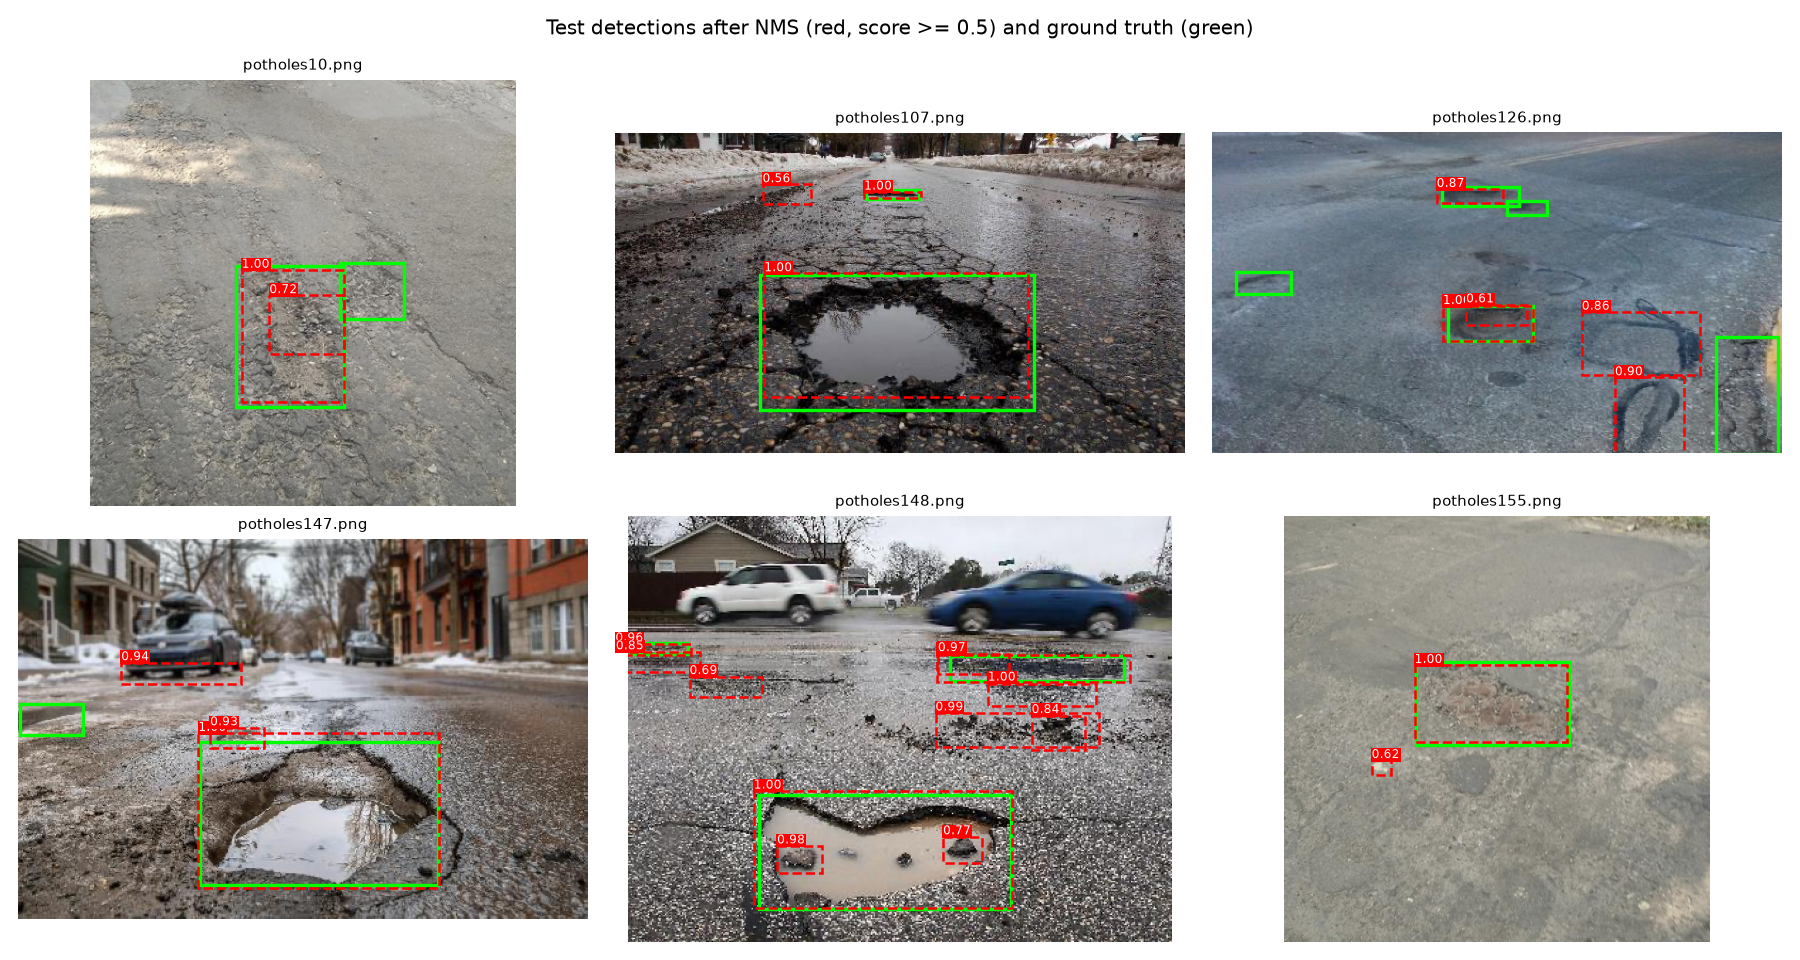
\includegraphics[width=\linewidth]{test_detections.png}
\caption{Test detections after NMS with score $\ge 0.5$ (red) and GT (green).}
\label{fig:det}
\end{figure}

The test detections (\cref{fig:det}) show three main failure modes: pothole-like regions such as patched asphalt or cracks get high scores; small boxes inside a large pothole (\eg stones in a puddle) have low IoU with the large box and survive NMS (the NMS failure case for overlapping objects); and 8\% of the test potholes are never covered by a proposal.

\noindent\textbf{Discussion.}
The results separate the two error sources of the detector. Classification is good: the proposal-level AP on the validation set is 0.92, and the precision-recall curve in \cref{fig:pr} stays above 0.8 precision up to about 50\% recall. Localisation is the bottleneck: box regression raises the mean IoU of the positive validation proposals with their GT box from 0.67 to 0.80, and the share with IoU $\ge 0.7$ from 38\% to 81\%. Hence regression helps most at IoU 0.75.

\noindent\textbf{Limitations.}
The model is trained with a single seed, and the test set has only 179 potholes, so differences of a few AP points should be interpreted with care. Classifying every proposal separately is slow compared with Fast R-CNN.

%--------------------------------------------------------------------
\section{Conclusion}
Selective Search in quality mode with 2000 proposals per image covers 92\% of the potholes, compared with 86\% for the fast mode. A ResNet-50 fine-tuned with a balanced sampler classifies the proposals with 92.7\% balanced accuracy despite a 25:1 imbalance. On the test set, NMS is essential (AP@0.5 0.067 $\to$ 0.585), and box regression raises AP@0.5 to 0.660 and triples AP@0.75.

%--------------------------------------------------------------------
\section{Use of AI}
Generative AI tools (Claude Code) were used extensively in this project: to write and debug the code, to run the experiments on the HPC cluster, and to draft the text of this report. All results were checked by the group, and the NMS and AP implementations were verified against \texttt{torchvision} and hand-computed examples.

\end{document}
